% !TEX root = ./main.tex


\section{Supplemental Information}

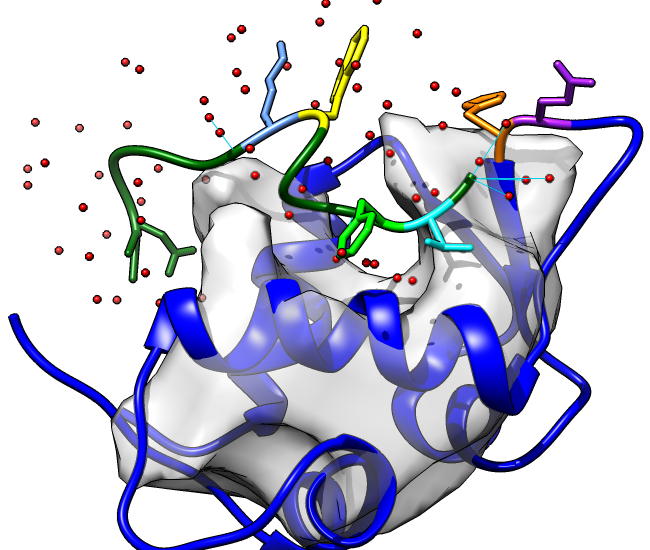
\includegraphics[width=3.03704in,height=2.40229in]{media/image6.tiff}\includegraphics[width=3.07837in,height=2.38889in]{media/image7.tiff}

\textbf{Figure S1.} Side-by-side comparison of MSMs constructed from
protein Cα and Cβ pair distances (left), and solvent shell features
(right), projected onto the first and second tICA components.

\includegraphics[width=6.5in,height=5.41806in]{media/image8.tiff}

Figure S2. \textbf{Solvent shells around key residues contribute to the
slowest motions.} (Top) The degree of contribution for each solvent
shell. Significant slow-dynamical solvent features are labeled by carbon
atom and residue to which it belongs. The green and blue slices denote
groups of residues for p53 and MDM2, respectively.~ (Bottom) The flux of
significant solvent dynamics relative to distinct solvent shells are
represented by pink (solvation) and yellow dots (de-wetting).

The second eigenvector revealed first shell (0-3 Å) of Methionine, M62
(β), Q71 (β), Q72 (α), Phenylalanine, F91 (β) of MDM2 as well as
Leucine, L25 (β), K24 (β) of p53 as the features contributing to the
slowest motions.

Movies:

RUN9\_CLONE70: (531 ns)

{[}This movie is the overlaid trajectory in Figure 4.{]}

\#RUN7\_CLONE41: (271 ns)

This bound-unfolded trajectory shows W23 (yellow) pointing into the page
when the position of the trajectory trace contains a negative tIC2
value. Likewise, tIC1 is also negative, and the surface buckles inside
the hydrophobic pocket leaving a large cavity. This cavity represents a
high volume of water inside the pocket.

Here, we can see that movement along tIC1 correlates to the distance
from the pocket i.e., displacement of water inside the pocket. The helix
begins to coil at S20 of p53 at 193 ns (00:06) pulling F19 (light green)
closer to the pocket, simultaneously increaing tIC1 on the tICA
landscape. The maximum tIC1 value correlates to the instant (232 ns) W23
and F19 both enter the pocket.

\#RUN13\_CLONE53: (2001 ns)

During the first 20.0 ns the conformation of p53 is folded-unbound. This
particular trajectory is very interesting, in that, when W23 enters the
pocket, it's unable to lock into place due to its crooked positioning
(00:15).

Eventually, large survace cavities begin to form, and W23 gets jostled
out and performs a 360° turn at 41.1 ns (00:16). The helix stabilizes
when W23 and F19 are comfortable in the pocket.

\#RUN15\_CLONE32: (851 ns)

\#RUN18\_CLONE96: (216 ns)

This short trajectory

\#RUN24\_CLONE68: (321 ns)